\documentclass[15pt]{beamer}
  
\newcommand\blfootnote[1]{%
  \begingroup
  \renewcommand\thefootnote{}\footnote{#1}%
  \addtocounter{footnote}{-1}%
  \endgroup
  }
%
% Choose how your presentation looks.
%
% For more themes, color themes and font themes, see:
% http://deic.uab.es/~iblanes/beamer_gallery/index_by_theme.html
%
\mode<presentation>
{
  \usetheme{default}      % or try Darmstadt, Madrid, Warsaw, ...
  \usecolortheme{default} % or try albatross, beaver, crane, ...
  \usefonttheme{default}  % or try serif, structurebold, ...
  \setbeamertemplate{navigation symbols}{}
  \setbeamertemplate{caption}[numbered]

} 

\usepackage[english]{babel}
\usepackage[utf8x]{inputenc}
\usepackage[absolute,overlay]{textpos}
\usepackage{amsmath}
\usepackage{lipsum}


\title[Your Short Title]{Bifurcation analysis of microbiome steady states}
\author{Zipeng Wang\\ Jean Carlson\\ Eric Jones\\ Josh Mueller}
\institute{UCSB}
\date{September 7,  2018}

\begin{document}

\begin{frame}
  \titlepage
\end{frame}

% Uncomment these lines for an automatically generated outline.
%\begin{frame}{Outline}
%  \tableofcontents
%\end{frame}

\section{Introduction}

\begin{frame}{General Goal}
%%%%%%%%%%%%%%%%%%%%slide1
\begin{columns}
\column{0.5\textwidth}
\begin{itemize}
	\item Modify diseased states into healthy states
	\item Ecology $\leftrightarrow$ Microbiome
	\item Change microbial interactions
\end{itemize}
 
\column{0.5\textwidth}
	\begin{textblock*}{6.8cm}(6.5cm,3cm) % {block width} (coords)
	 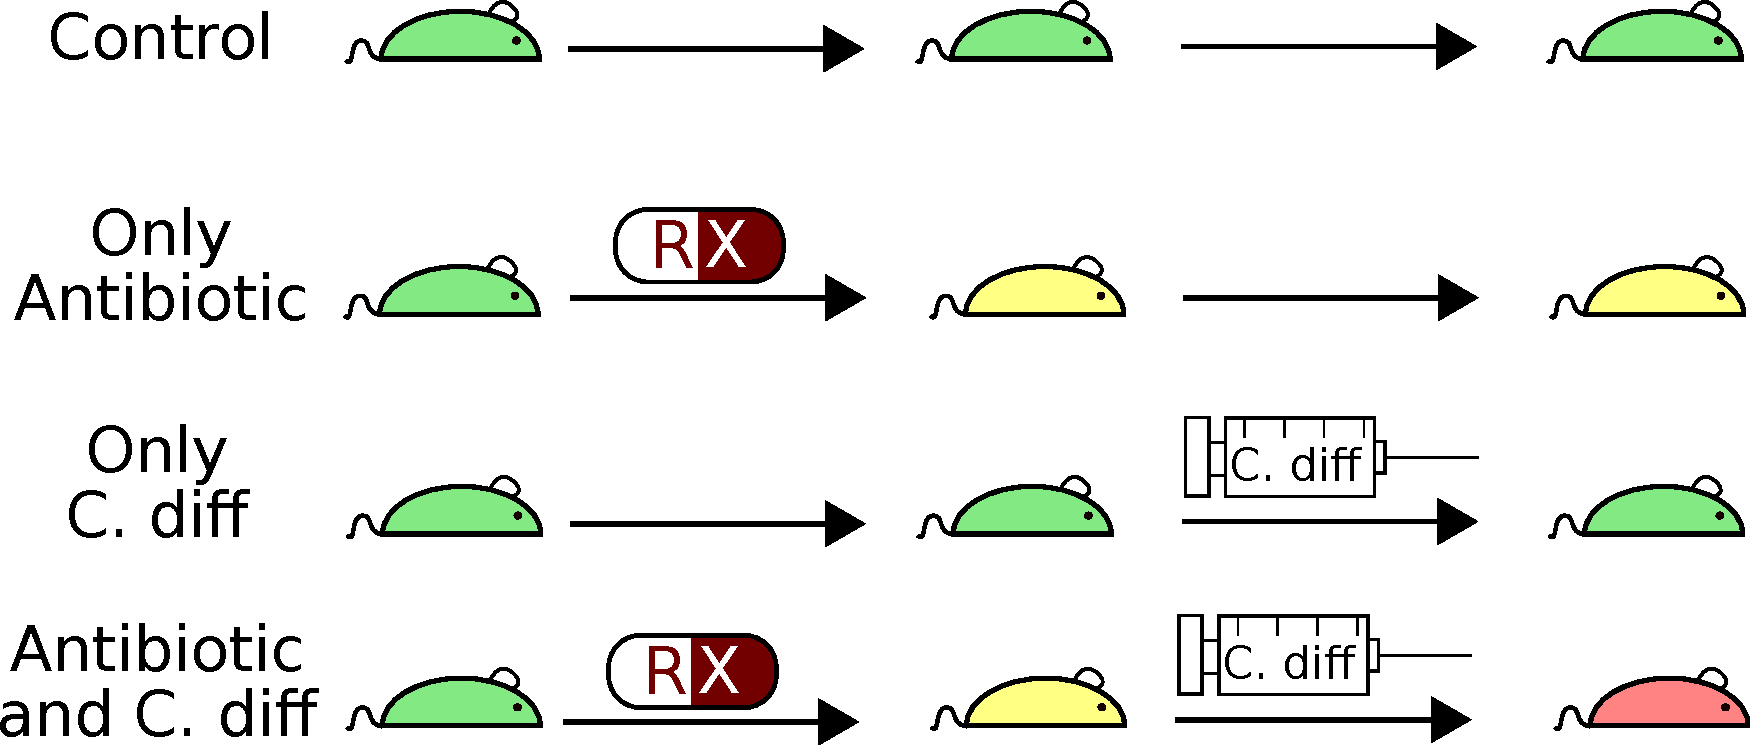
\includegraphics[width=0.9\textwidth]{mouse_final}\\[-1ex]
	 {\tiny }
	\end{textblock*}
\end{columns}
\end{frame}

%%%%%%%%%%%%%%%%%%%%slide1.5
\begin{frame}{General Goal}
\begin{columns}
\column{0.5\textwidth}
\begin{itemize}
	\item Modify diseased states into healthy states
	\item Ecology $\leftrightarrow$ Microbiome
	\item Change microbial interactions
\end{itemize}
 
\column{0.5\textwidth}
	\begin{textblock*}{6.8cm}(6.5cm,2cm) % {block width} (coords)
	 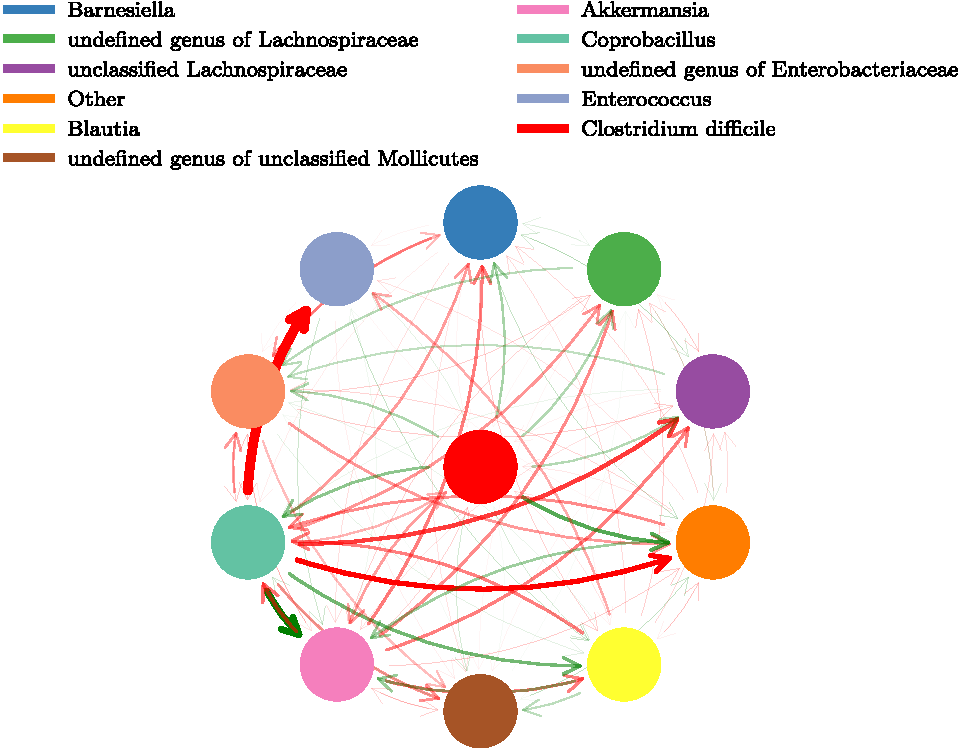
\includegraphics[width=0.9\textwidth]{food_web_w_legend_preplos}\\[-1ex]
	 {\tiny Source: Jones and Carlson, PLoS Comp. Biol. 2018}
	\end{textblock*}
\end{columns}
\end{frame}

%%%%%%%%%%%%%%%%%%%%slide2
\begin{frame}{General Goal}
\begin{columns}
\column{0.5\textwidth}
\begin{itemize}
	\item Modify diseased states into healthy states
	\item Ecology $\leftrightarrow$ Microbiome
	\item Change microbial interactions
	\item Example: change acidity of environment
\end{itemize}
 
\column{0.5\textwidth}
	\begin{textblock*}{6.8cm}(6.5cm,2cm) % {block width} (coords)
	 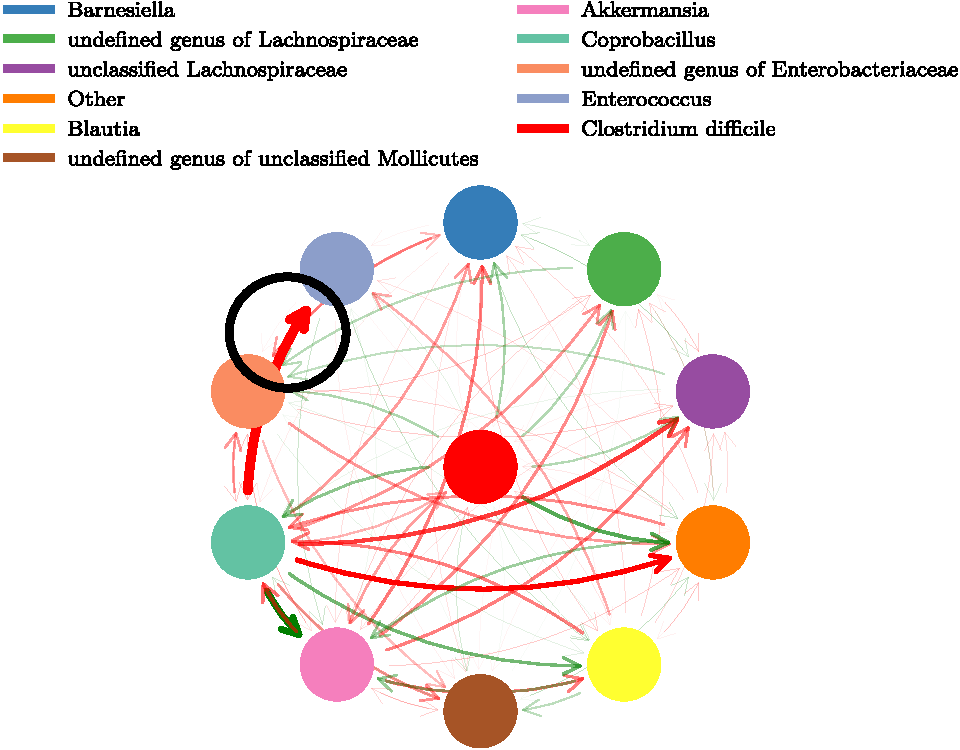
\includegraphics[width=0.9\textwidth]{food_web_w_circle}\\[-1ex]
	 {\tiny Source: Jones and Carlson, PLoS Comp. Biol. 2018}
	\end{textblock*}
\end{columns}
\end{frame}

%%%%%%%%%%%%%%%%%%%%slide3
\begin{frame}{Stein Model}
\begin{columns}
\column{0.5\textwidth}
\begin{itemize}
	\item Based on experiments
	\item 11 categories; 11-D vector
\end{itemize}

\column{0.5\textwidth}
	\begin{textblock*}{6.8cm}(6.5cm,2cm) % {block width} (coords)
	 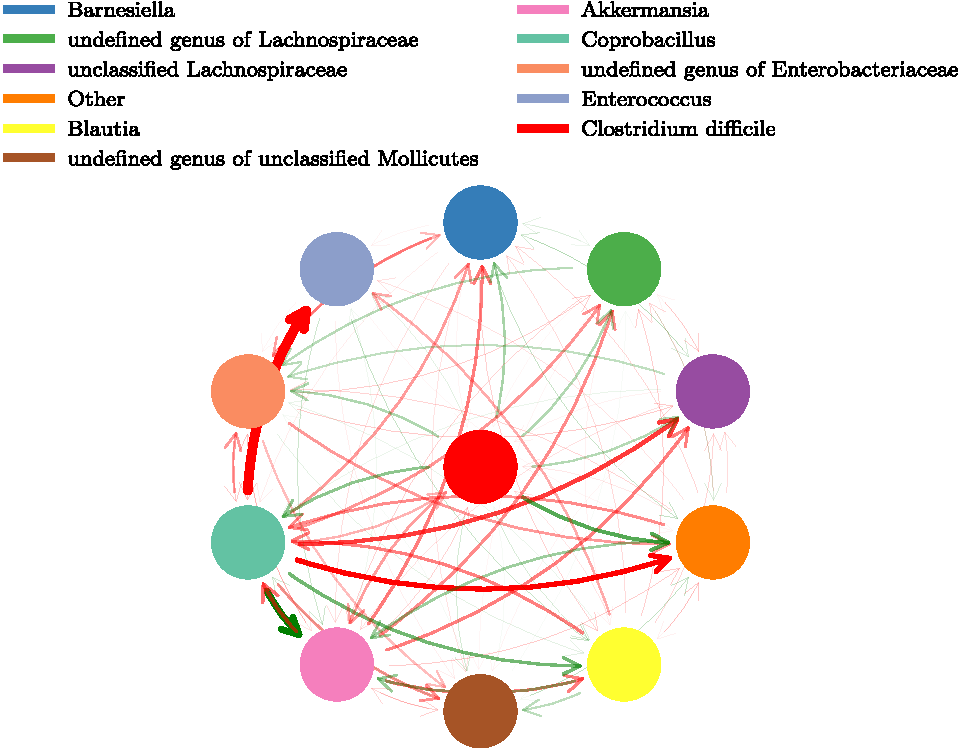
\includegraphics[width=0.9\textwidth]{food_web_w_legend_preplos}\\[-1ex]
	 {\tiny Source: Jones and Carlson, PLoS Comp. Biol. 2018}
	\end{textblock*}
\end{columns}
\end{frame}




%%%%%%%%%%%%%%%%%%%%slide4]
\begin{frame}{Generalized Lotka-Volterra equations}
Taylor Expansion:
\begin{eqnarray*}
\frac{d\vec{y}}{dt} = f(\vec{y}) &\approx& f(\vec{0})+ Df(\vec{0})\cdot \vec{y}+ \vec{y}^T \cdot Hf(\vec{0})\cdot \vec{y}\\
\end{eqnarray*}
N-species gLV Equations:
\begin{eqnarray*}
\frac{d}{dt}y_i(t) &=& y_i(t)\Big(\color{blue} \rho_i \color{black} + \sum_{j=1}^N \color{red} K_{ij} \color{black} y_i(t)\Big)
\end{eqnarray*}


2D: 

\[
 \begin{cases}
       \frac{dx_a}{dt} = \color {blue} \overbrace{\mu_a} \color{black} x_a -\color{red}\overbrace{M_{aa}\color{black} x_a^2- \color{red}M_{ab} \color{black} x_a x_b}\\
       \frac{dx_b}{dt} = \color {blue}\mu_b\color{black} x_b-\color{red}M_{ba}\color{black}x_ax_b-\color{red}M_{bb}\color{black}x_b^2\\
 \end{cases}
\]
\begin{textblock*}{6cm}(4.2cm,6.8cm) % {block width} (coords)
\color{blue} growth rate
\end{textblock*}
\begin{textblock*}{6cm}(6.8cm,6.8cm) % {block width} (coords)
\color{red} interaction \color{black}
\end{textblock*}
\end{frame}


%%%%%%%%%%%%%%%%%%%%slide6
\begin{frame}{Dynamical Landscape}
\begin{columns}
\column{0.5\textwidth}

\begin{textblock*}{6cm}(1cm,1.2cm)
Equivalent form:
\[
 \begin{cases}
       \frac{dx_a}{dt} = x_a(1-x_a-M_{ab}x_b)\\
       \frac{dx_b}{dt} = x_b(\mu_b-M_{ba}x_a-x_b)\\
 \end{cases}
\]
Taking $\mu_b = 1$:
\end{textblock*}
\column{0.5\textwidth}
\begin{textblock*}{10cm}(3.4cm,3.1cm) % {block width} (coords)
	 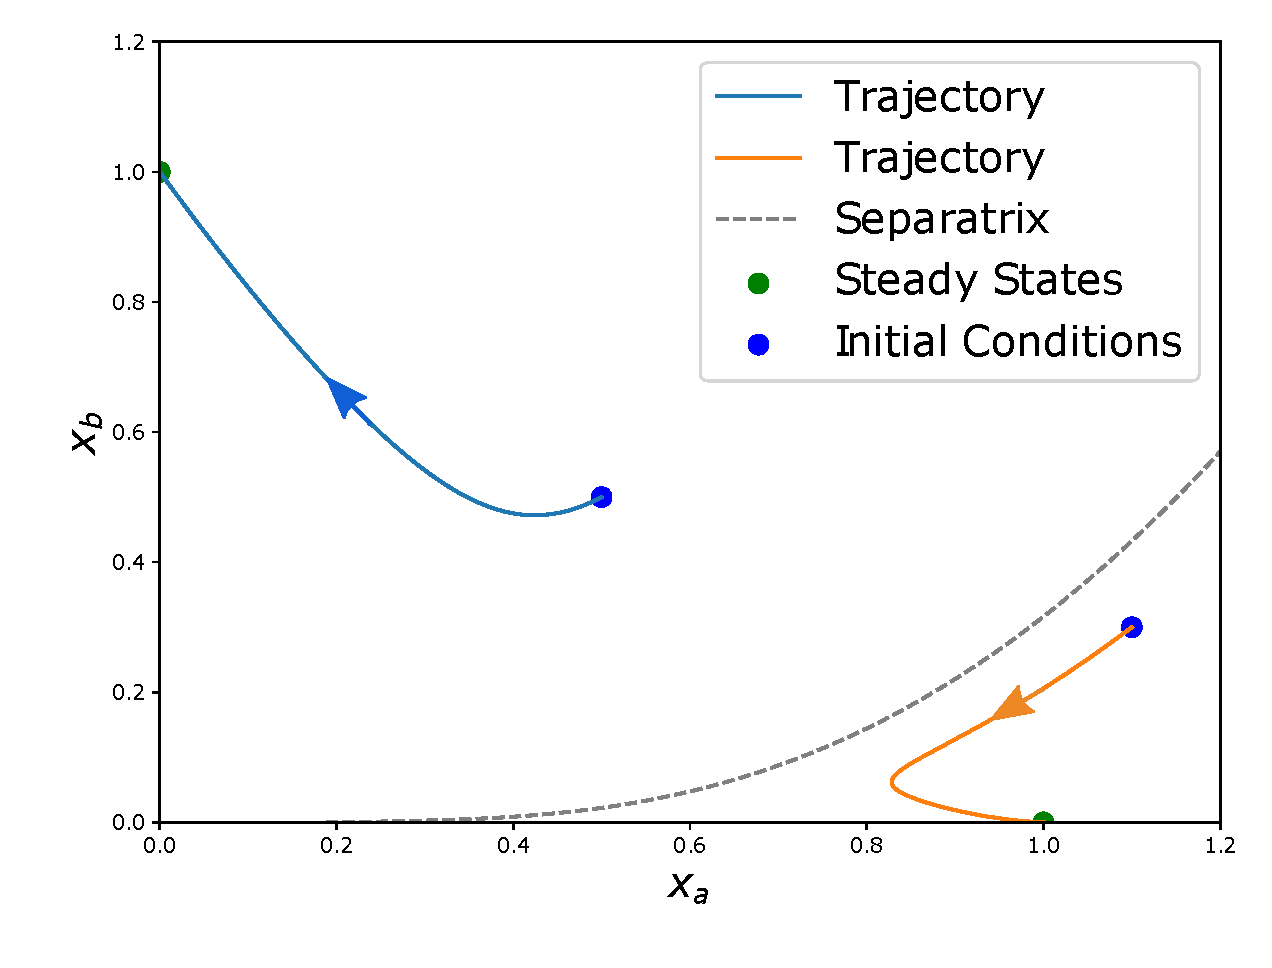
\includegraphics[width=0.9\textwidth]{example_plot}\\
	\end{textblock*}
\end{columns}
\end{frame}






\section{Results}
%%%%%%%%%%%%%%%%%%%%slide8
\begin{frame}{Project Goal}
\begin{columns}
\column{0.5\textwidth}
\begin{itemize}
	\item Consider steady states C and E
	\item Start at the middle point
	\item Use SSR to reduce K to M
	\item Modify interaction matrix M 
	\item Change system from C to E
\end{itemize}

\column{0.5\textwidth}
	\begin{textblock*}{6cm}(6.5cm,2cm) % {block width} (coords)
	 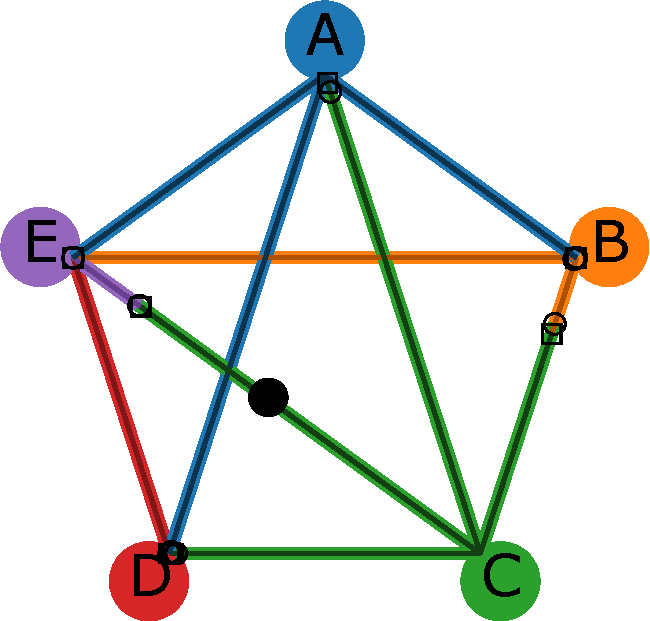
\includegraphics[width=0.9\textwidth]{attractor_network_v3_w_dot}
	\end{textblock*}
\end{columns}
\end{frame}

%%%%%%%%%%%%%%%%%%%%slide9
\begin{frame}{Original Trajectory}
	\begin{textblock*}{12cm}(1cm,1cm) % {block width} (coords)
	 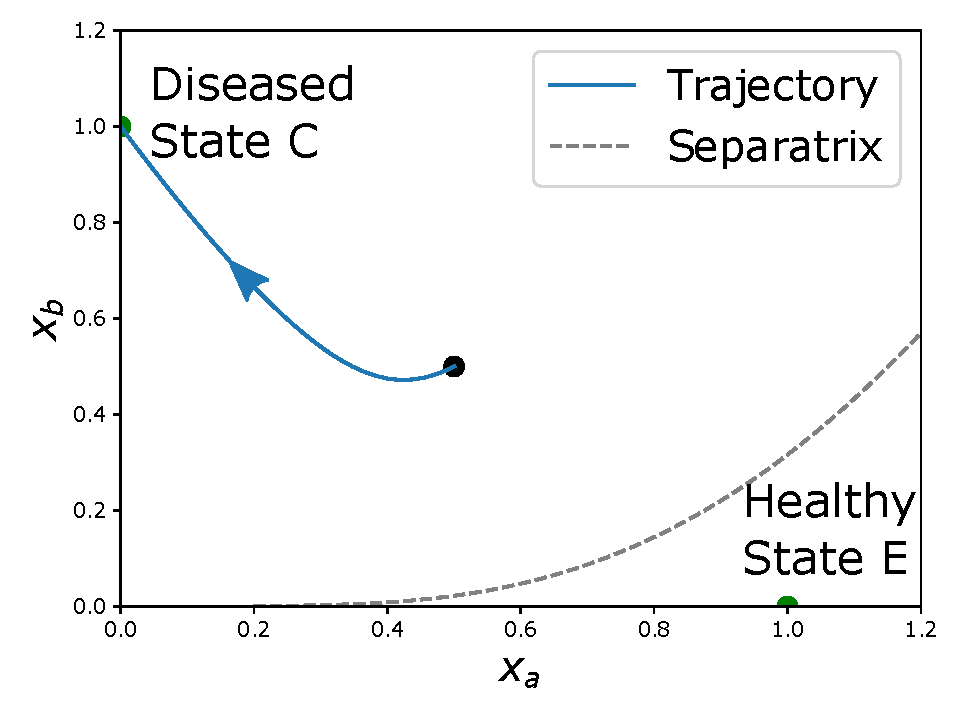
\includegraphics[width=0.9\textwidth]{original}
	\end{textblock*}
\end{frame}

%%%%%%%%%%%%%%%%%%%%slide10
\begin{frame}{Bifurcation Analysis}

\begin{columns}
\column{0.5\textwidth}
\begin{itemize}
	\item Separatrix moves with the third steady state
	\item Originally in upper right region
	\item going towards upper left
\end{itemize}
\column{0.5\textwidth}
	\begin{textblock*}{7.6cm}(5.5cm,1cm) % {block width} (coords)
	 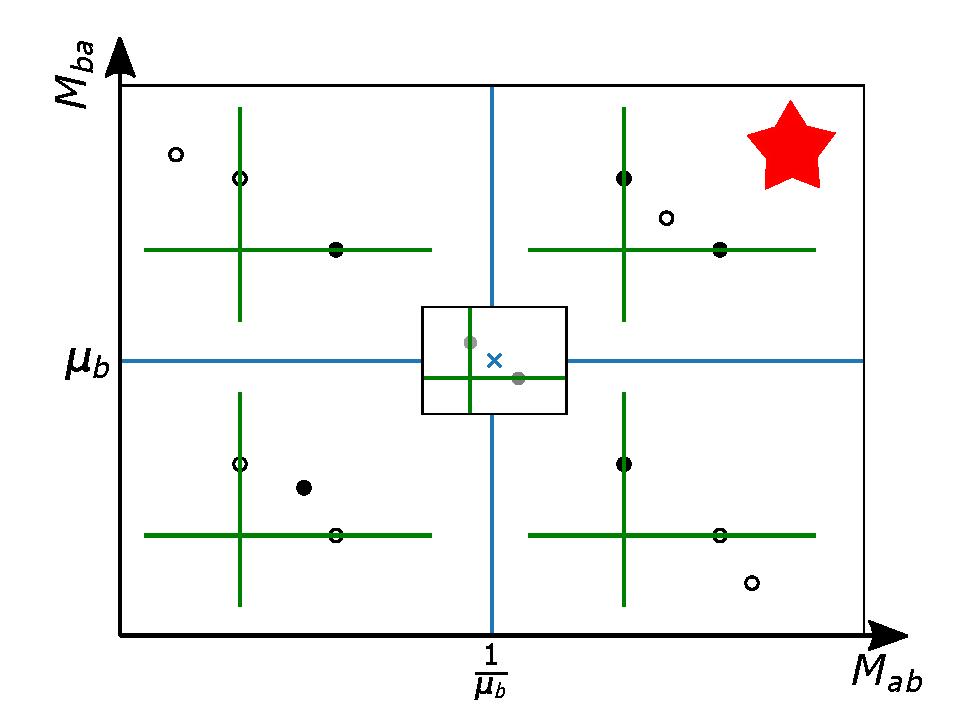
\includegraphics[width=0.9\textwidth]{bifurcation}
	 {\small
	  Black dots shows stable steady states, and \\hollow dots shows unstable steady states}
	\end{textblock*}
\end{columns}
\end{frame}

%%%%%%%%%%%%%%%%%%%%slide11
\begin{frame}{Change in M}
\begin{columns}
\column{0.5\textwidth}
\begin{textblock*}{7cm}(0cm,1.3cm) % {block width} (coords)
	 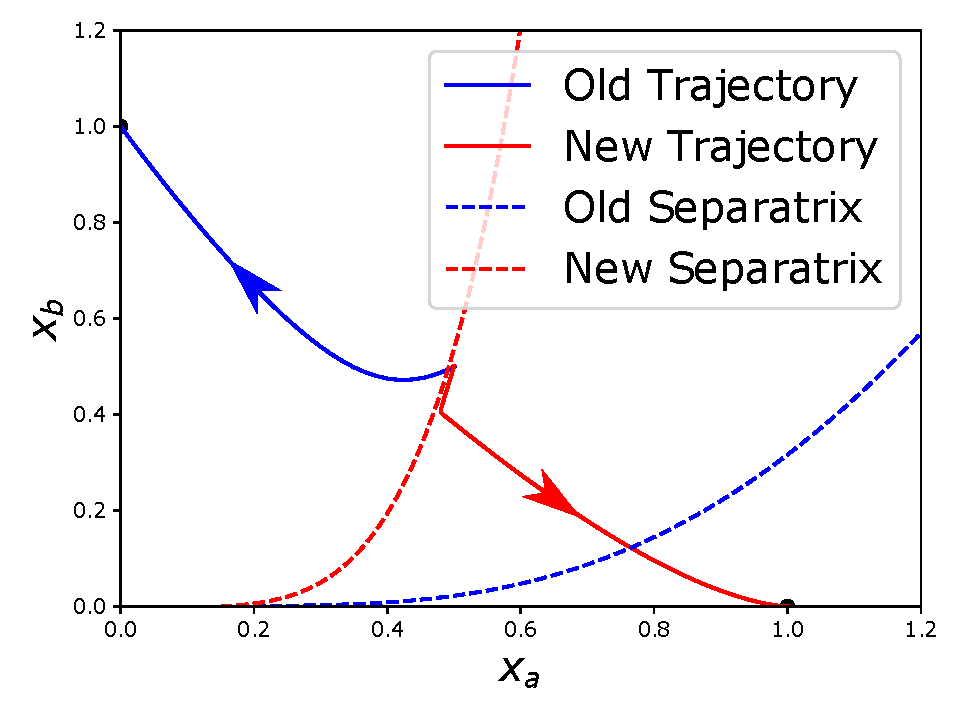
\includegraphics[width=0.9\textwidth]{changed_traj_sep}
	\end{textblock*}
\column{0.5\textwidth}
	\begin{textblock*}{7.3cm}(6.2cm,1cm) % {block width} (coords)
	 \includegraphics[width=0.9\textwidth]{delta_M_PARA}
	\end{textblock*}
\end{columns}
\begin{textblock*}{6cm}(1.4cm,6.2cm) % {block width} (coords)
Microbial Phase Space
\end{textblock*}
\begin{textblock*}{6cm}(8.2cm,6.2cm) % {block width} (coords)
Parameter Space
\end{textblock*}
\end{frame}

%%%%%%%%%%%%%%%%%%%%slide7.5
\begin{frame}{Steady State Reduction(SSR)}
\begin{columns}
\column{0.5\textwidth}
\begin{textblock*}{6cm}(1cm,2cm) % {block width} (coords)
	 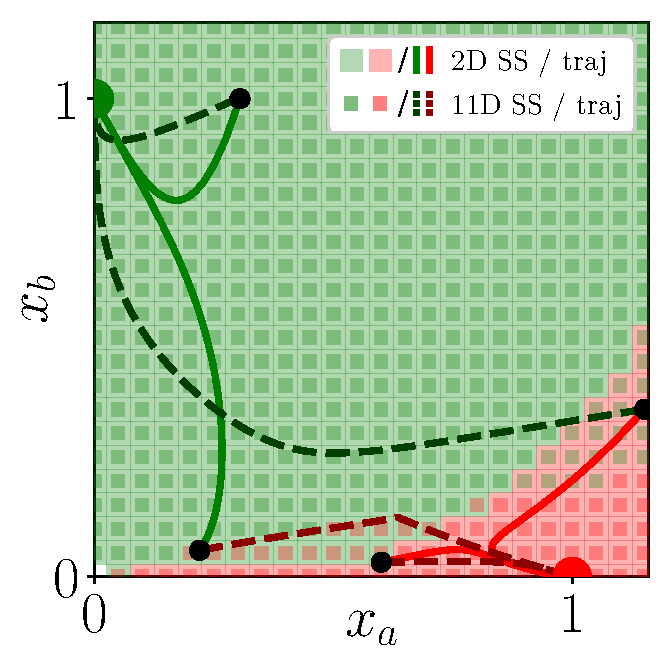
\includegraphics[width=0.9\textwidth]{fig4_no_inset_v0}\\[-1ex]
	 {\tiny Source: Jones and Carlson, arXiv:1808.01715}
	\end{textblock*}

\column{0.5\textwidth}
	\begin{textblock*}{6cm}(6.8cm,1.7cm) % {block width} (coords)
	 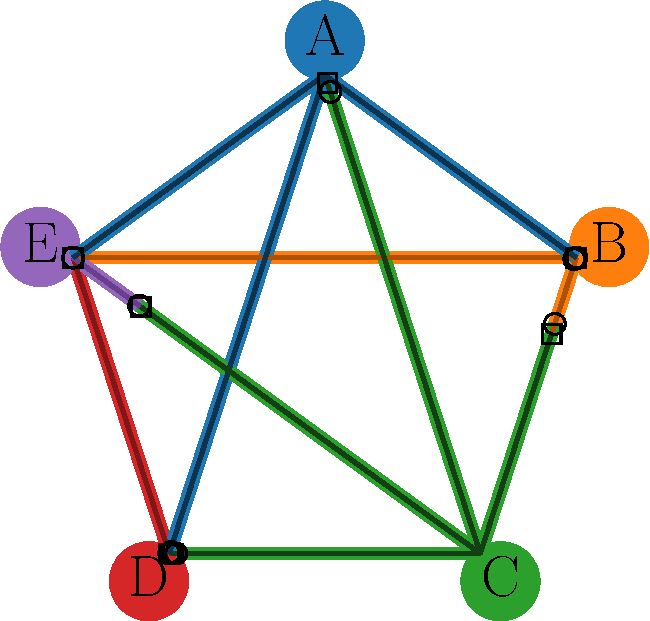
\includegraphics[width=0.9\textwidth]{attractor_network_v3}
	 {A-E: Steady states\\ Circle and square: Separatrices predicted by 11-D model and 2-D model}
	\end{textblock*}
\end{columns}
\end{frame}

%%%%%%%%%%%%%%%%%%%%slide7
\begin{frame}{Steady State Reduction(SSR)}
\begin{columns}
\column{0.55\textwidth}
\begin{align*}
\mu_\gamma &= \vec{\rho} \cdot \vec{y_\gamma}\\
M_{\gamma \delta} &= \vec{y_\gamma}^T K \vec{y_\delta}\\
      \gamma,\delta &\in a,b
\end{align*}

\begin{itemize}
	\item Simplify 11-D to 2-D
	\item Works well for Stein model
\end{itemize}

\column{0.45\textwidth}
	\begin{textblock*}{6cm}(6.8cm,1.7cm) % {block width} (coords)
	 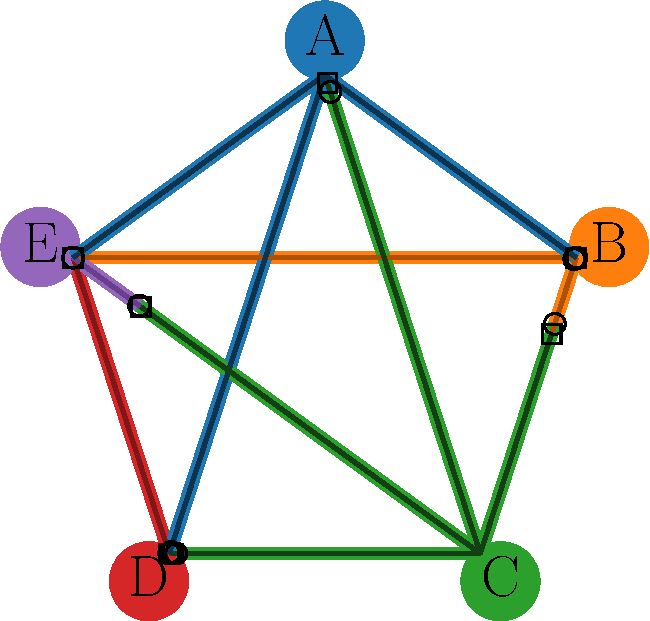
\includegraphics[width=0.9\textwidth]{attractor_network_v3}
	 {A-E: Steady states\\ Circle and square: Separatrices predicted by 11-D model and 2-D model}
	\end{textblock*}
\end{columns}
\end{frame}

%%%%%%%%%%%%%%%%%%%%slide12
\begin{frame}{Change in K}
\begin{columns}
\column{0.45\textwidth}
\begin{align*}
M_{ab} &= \vec{y_a}^T K \vec{y_b}\\
	   &= \sum_{i=1,j=1}^{11,11} \alpha_{ij}K_{ij}
\end{align*}

\begin{itemize}
	\item 121 coefficients
	\item Most are 0
	\item $M_{ab}$ most sensitive to change in $k_{ij}$ with the largest $\alpha_{ij}$ coefficient
\end{itemize}

\column{0.45\textwidth}
	\begin{textblock*}{8cm}(5.5cm,2cm) % {block width} (coords)
	 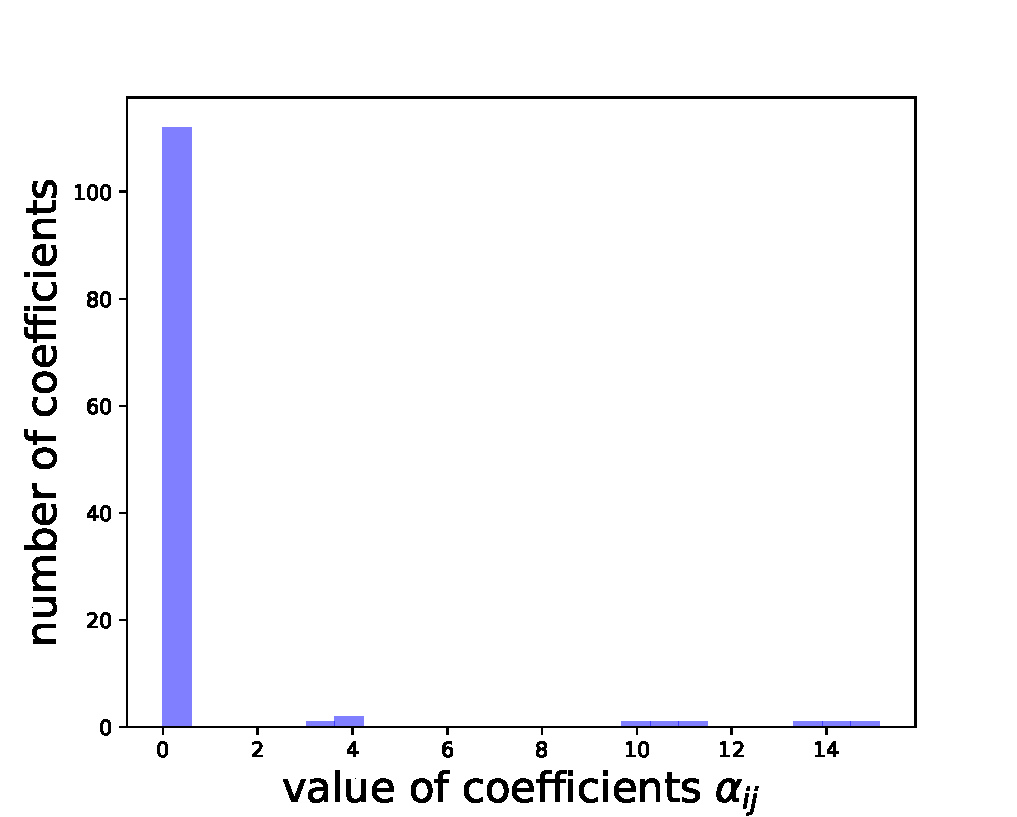
\includegraphics[width=0.9\textwidth]{hist}
	\end{textblock*}
\end{columns}
\end{frame}

%%%%%%%%%%%%%%%%%%%%slide13
\begin{frame}{11-D Trajectory}
\begin{columns}
\column{0.4\textwidth}
\begin{itemize}
	\item 11-D Trajectory projected to plane spanned by SSC and SSE 
	\item It works!
\end{itemize}

\column{0.6\textwidth}
	\begin{textblock*}{9cm}(5cm,1cm) % {block width} (coords)
	 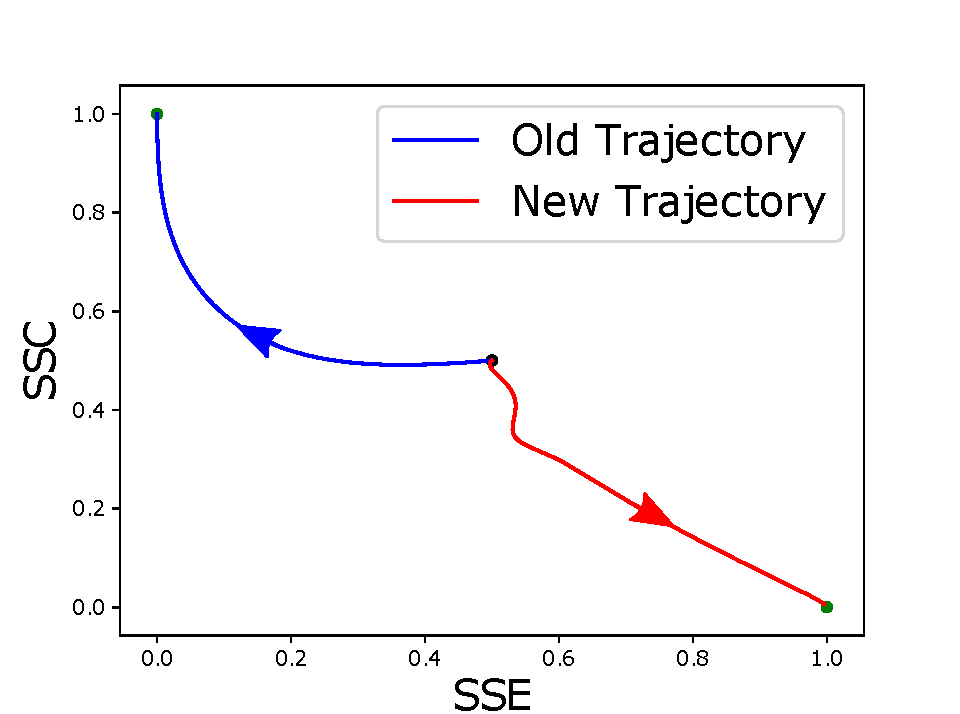
\includegraphics[width=0.9\textwidth]{11-D_traj}
	\end{textblock*}
\end{columns}
\end{frame}

%%%%%%%%%%%%%%%%%%%%slide13
\begin{frame}{11-D Trajectory}
\begin{columns}
\column{0.4\textwidth}
\begin{itemize}
	\item 11-D Trajectory projected to plane spanned by SSC and SSE 
	\item It works!
\end{itemize}

\column{0.6\textwidth}
	\begin{textblock*}{7cm}(6cm,1cm) % {block width} (coords)
	 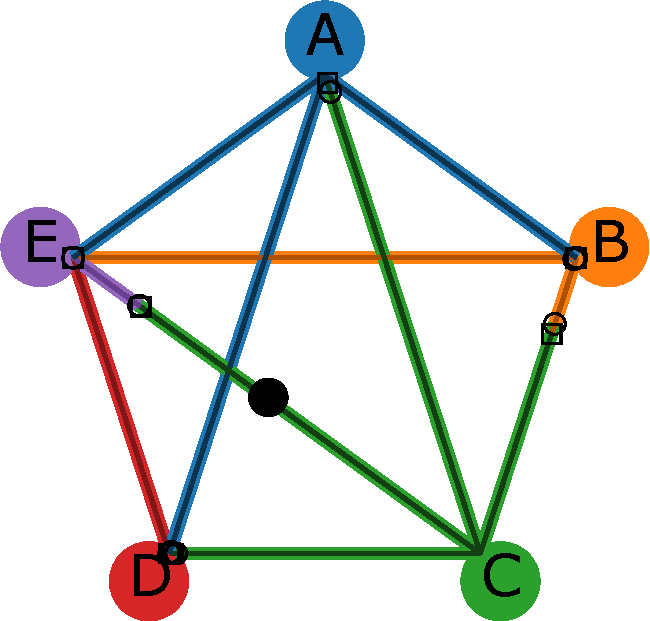
\includegraphics[width=0.9\textwidth]{attractor_network_v3_w_dot}
	\end{textblock*}
\end{columns}
\end{frame}

%%%%%%%%%%%%%%%%%%%%slide13
\begin{frame}{11-D Trajectory}
\begin{columns}
\column{0.4\textwidth}
\begin{itemize}
	\item 11-D Trajectory projected to plane spanned by SSC and SSE 
	\item It works!
\end{itemize}

\column{0.6\textwidth}
	\begin{textblock*}{7cm}(6cm,1cm) % {block width} (coords)
	 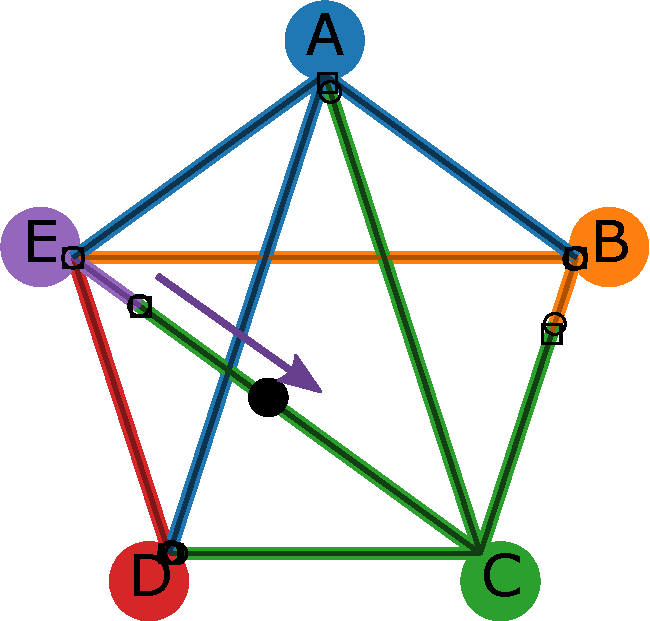
\includegraphics[width=0.9\textwidth]{attractor_network_v3_w_arrow}
	\end{textblock*}
\end{columns}
\end{frame}

%%%%%%%%%%%%%%%%%%%%slide14
\begin{frame}{Summary}
\setbeamertemplate{bibliography item}{}
\begin{thebibliography}{99} 
\bibitem[Jones and Carlson, PLoS Comp. Biol. 2018]{1}   
\bibitem[Jones and Carlson, arXiv:1808.01715]{2}   
\end{thebibliography}
\begin{itemize}
	\item Reduce to 2-D; use bifurcation analysis to guide; project to 11-D
	\item Can be applied to other complex system with favorable and unfavorable steady states such as...
	\begin{itemize}
	\item Gene regulatory networks
	\item Neural networks
	\end{itemize}

	\item Questions?
\end{itemize}
\blfootnote{Acknowledgement: Jean Carlson; Eric Jones;
Josh Mueller}
\end{frame}


\end{document}
